\subsection{Modelling}
หลังจากที่เราได้ออกแบบและโมเดลหุ่นยนต์ของเราขึ้นมาที่ใช้ CAD tools ต่างๆ เช่น AutoCAD, SolidWorks, Blender
หรืออื่นๆ ก็เพื่อที่จะนำมาใช้ในการทำ Simulation การที่เราทำ Simulation นั้นก็จะสามารถมองเห็นหุ่นยนต์
และเห็นการทำงานของหุ่นยนต์เราก่อนที่เราจะสร้างมันขึ้นมาจริงๆ หุ่นยนต์จำลองที่เราสร้างขึ้นมานั้นควรที่จะมีลักษณะให้ใกล้เคียงกับของจริงมากที่สุด
ไม่ว่าจะเป็นรูปร่าง รูปทรง น้ำหนักต่างๆ 

\subsubsection{ROS packages for robot modelling}
ROS นั้นได้ให้เครื่องมือที่ช่วยให้เราสามารถสร้าง 3D robot models ได้
ใน ROS มี meta package ที่ชื่อว่า robot\_model ซึ่งข้างในมี package ต่างๆที่ใช้สำหรับสร้าง 3D robot models
        
\paragraph*{urdf}
เป็น 1 ในหลายๆ package ที่อยู่ใน robot\_model, urdf เป็น xml ไฟล์ที่เอาไว้ใช้บอกลักษณะของหุ่นยนต์ ย่อมาจาก Unified Robot Description Format(URDF)
เราสามารถระบุ robot model, sensors และ working environment โดยใช้ URDF การบอกนั้นจะสามารถบอกเป็นเหมือน tree structure ของ link ต่างๆในตัวหุ่นยนต์ สามารถบอก rigid link เชื่อมต่อกันผ่าน joints แต่ถ้าเป็น flexible link จะไม่สามารถบอกได้โดยใช้ urdf

\subparagraph*{joint\_state\_publisher}
เครื่องมือนี้มีประโยชน์มากในการ model robot URDF เพราะมันสามารถหา joints ทุก joint ที่ไม่ใช่ fixed joints มาแสดงเป็น GUI sliders ทำให้เราสามารถเลื่อนๆหมุนๆไปมาได้ อีกทั้งยังสามารถใช้งานร่วมกับ visualize RViz

\subparagraph*{robot\_state\_publisher}
เป็นเครื่องมือที่ใช้ในการ publish 3d pose ของ link ต่างๆใน urdf การ ยublish นั้นจะใช้ ROS tf(transform) ROStf คือการหาความสัมพันธ์ระหว่าง frame ของหุ่นยนต์

\subparagraph*{xacro}
ย่อมาจาก XML Macros หรือเราสามารถเรียกอีกอย่างว่า URDF plus add-ons. ซึ่งการทำงานเหมือนกับ urdf แต่ทำให้ไฟล์ urdf สั้นกว่า อ่านง่ายกว่า และสามารถใช้เพื่อทำให้สร้างหุ่นยนต์ที่มีความซับซ้อนง่ายขึ้น เราสามารถแปลงไฟล์ xacro เป็น urdf ได้

\subsubsection{URDF}
ในส่วนนี้จะเป็นการอธิบายระบบทางกลของหุ่นยนต์ฮิวมานอยด์เป็นไฟล์ที่ใช้ร่วมกับ ROS ได้ เพื่อที่จะสามารถนำไปใช้กับ Simulation ในอนาคตได้
ในการอธิบายระบบทางกลนั้นผู้วิจัยได้ใช้ไฟล์ URDF (Universal Robotics Description Format) ซึ่งใช้ภาษาการเขียนเป็น XML ในการบอกส่วนประกอบแต่ละส่วนของหุ่นยนต์

\subsubsection*{Link}
ในไฟล์ URDF แต่ละชิ้นส่วนของหุ่นยนต์เราจะเรียกว่า link แล้วใน link จะประกอบไปด้วยส่วนย่อยๆ
3 ส่วนคือ <inertia> ที่เอาไว้บอกถึงค่าตัวแปรทางฟิสิกส์, <visual> ที่เอาไว้แสดงผลให้เราเห็น, 
<collision> ที่เอาไว้ตรวจสอบว่าหุ่นยนต์มีการชนกันกับสิ่งแวดล้อมไหม ดังรูปที่ \ref{fig:urdf_link_code}

\clearpage
\begin{figure}[ht]
\begin{Verbatim}[fontsize=\small]
<link name="my_link">
    <inertia>
        <origin xyz="0 0 0.5" rpy="0 0 0"/>
        <mass value="1"/>
        <inertia ixx="100" ixy="0" ixz="0" iyy="100" iyz="0" izz="100"/>
    </inertia>
    <visual>
        <origin xyz="0 0 0" rpy="0 0 0"/>
        <geometry>
            <box size="1 1 1" />
        </geometry>
        <material name="Cyan">
            <color rgba="0 1.0 1.0 1.0"/>
        </material>
    </visual>
    <collision>
        <origin xyz="0 0 0" rpy="0 0 0"/>
        <geometry>
            <cylinder radius="1" length="0.5"/>
        </geometry>
    </collision>
</link>
\end{Verbatim}
\caption{ตัวอย่าง link ใน urdf}
\label{fig:urdf_link_code}
\end{figure}

ยังมี tags อีกหลายตัวที่ใช่ในการอธิบายแต่ละชิ้นส่วนของหุ่นยนต์ แต่ตัวอย่างเป็นเพียงแค่ส่วนหนึ่งเท่านั้น
ในความเป็นจริงแล้วเราจะเขียน tags ต่างๆก็ตามที่เราต้องการ โดยใน URDF ไฟล์นั้นจะเอาไว้เก็บข้อมูลลักษณะเฉพาะของหุ่นยนต์เอาไว้
และยังสามารถใช้กับซอฟแวร์ตัวอื่นๆอีกได้

\begin{figure}[ht]
	\centering
	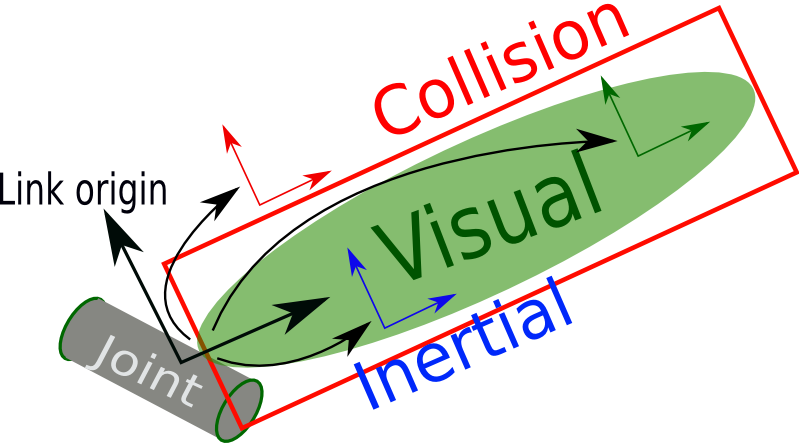
\includegraphics[width=0.60\textwidth]{chapter3/images/urdf_link.png}
	\caption{การอธิบาย link ใน URDF ไฟล์}
	\label{fig:urdf_link}
\end{figure}

\clearpage
\subsubsection*{Joint}
อีกส่วนที่สำคัญสำหรับการสร้างไฟล์หุ่นยนต์ด้วย URDF ก็คือ Joint tag โดย tag นี้จะอธิบายถึงความสัมพันธ์ระหว่างก้านต่อสองอัน
ส่วนนี้ไม่ได้มีเพียงแค่ทำข้อต่อให้เป็นแบบหมุนได้อย่างเดียว ยังมี Fix, Revolution, Linear และ Planar นอกเหนือจากนี้
เรายังสามารถที่จะเพิ่มองศาสูงสุดต่ำสุดของข้อต่อ รวมไปถึง dynamic properties ต่างๆ ตามที่เห็นดังรูปที่ \ref{fig:urdf_joint_code}
\begin{figure}[ht]
\begin{Verbatim}[fontsize=\small]
<joint name="my_joint" type="floating">
	<origin xyz="0 0 1" rpy="0 0 3.1416"/>
	<parent link="link1"/>
	<child link="link2"/>
	<calibration rising="0.0"/>
	<dynamics damping="0.0" friction="0.0"/>
	<limit effort="30" velocity="1.0" lower="-2.2" upper="0.7"/>
	<safety_controller k_velocity="10" k_position="15" 
	soft_lower_limit="-2.0" soft_upper_limit="0.5"/>
</joint>
\end{Verbatim}
\caption{ตัวอย่าง joint ใน urdf}
	\label{fig:urdf_joint_code}
\end{figure}

เมื่อเรานำ Joint และ Link มารวมกันเราจะต้องพิจารณาว่ามีวางรูปแบบเป็นไปตามรูปที่ \ref{fig:urdf_joint}
โดยจะมีระยะระหว่างแกนของแต่ละข้อต่อกับก้านต่อ ชิ้นส่วนแรกของการสร้างไฟล์ URDF จะมีชื่อว่า base\_link
และเฟรม origin จะเป็นเฟรมอ้างอิง เมื่อเราต่อ Joint เข้ากับ Link จะเรียกก้านต่อที่เอามาติดว่า parent
โดยเฟรม origin ของข้อต่อจะอยู่จุดเดียวกับเฟรม origin ของก้านต่อ ในสถานะเดียวกันก้านต่อที่นำมาต่อจากข้อต่อ
เราจะเรียกว่า child และเฟรม origin ของก้านต่อ child จะอยู่ที่จุดเดียวกับเฟรม origin ของข้อต่อ

\begin{figure}[h]
	\centering
	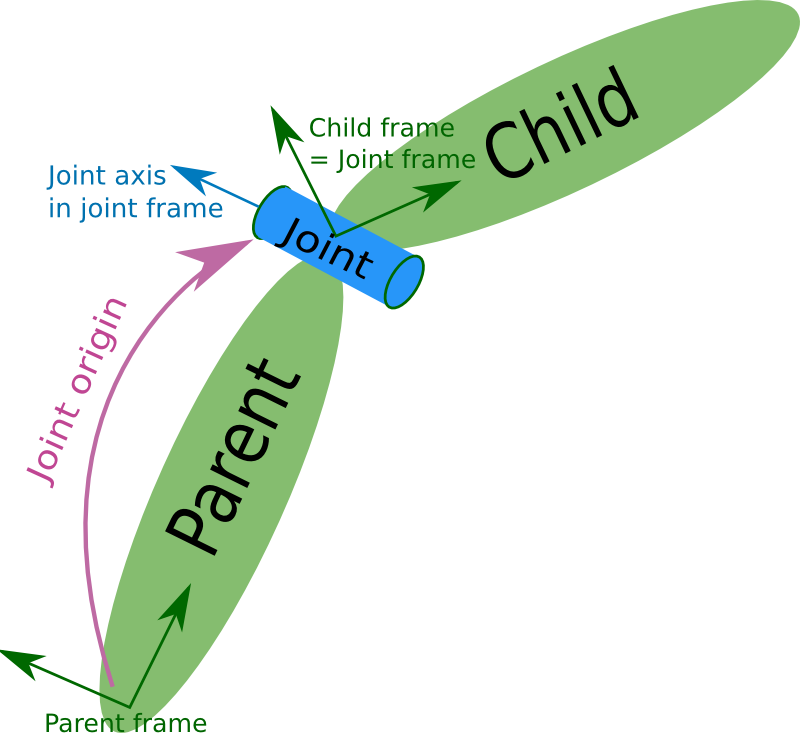
\includegraphics[width=0.55\textwidth]{chapter3/images/urdf_joint.png}
	\caption{การอธิบาย Joint ใน URDF ไฟล์}
	\label{fig:urdf_joint}
\end{figure}

\clearpage
\subsection{Box model}
